\documentclass[useAMS,usenatbib]{mnras}
\usepackage{color}
\usepackage{graphicx}
\usepackage{dcolumn}
\usepackage{bm}
\usepackage{amssymb}
\usepackage{latexsym}
\usepackage[T1]{fontenc}
\usepackage{aecompl} 

\newcommand{\hMsun}{{\ifmmode{h^{-1}{\rm
        {M_{\odot}}}}\else{$h^{-1}{\rm{M_{\odot}}}$~}\fi}} 
\newcommand{\hMpc}{{\ifmmode{h^{-1}{\rm Mpc}}\else{$h^{-1}$Mpc }\fi}}

%%%%%%%%%%%%%%%%%%%%%%%%%%%%%%%%%%%%%%%%%%%%%%%%

\begin{document}

\title[Constraining CPL via clustering shells of BOSS]{Cosmological constraints via clustering shells: 
constraining the Chevallier-Polarski-Linder parametrization using the SDSS-III BOSS data}

\author[Xiao-Dong~Li, Yuting Wang, Gong-bo Zhao, Changbom Park, Hyunbae Park, Cristiano G. Sabiu]
{ Xiao-Dong Li$^{1,2,\dagger}$,  Yuting Wang$^{2}$, Gong-bo Zhao$^{2}$, Changbom Park$^{1}$, Hyunbae Park$^{2}$, 
Cristiano G. Sabiu$^{2,\star}$, Juhan Kim$^{3,1}$\\
$^1$School of Physics, Korea Institute for Advanced Study, 85 Heogi-ro, Dongdaemun-gu, Seoul 130-722, Korea\\
$^2$Korea Astronomy and Space Science Institute, 776, Daedeokdae-ro, Yuseong-gu, Daejeon, 305-348, Korea\\
$^3$Center for Advanced Computation, Korea Institute for Advanced Study, 85 Hoegi-ro, Dongdaemun-gu, Seoul 130-722, Korea\\
$^{\dagger}$xiaodongli@kias.re.kr\\
$\star$Corresponding Author: csabiu@kasi.re.kr}




%\date{Accepted 1988 December 15. Received 1988 December 14; in original form 1988 October 11}

% \begin{keywords}
% methods: data analysis -- methods: statistical -- Galaxies:
% kinematics and dynamics -- Cosmology: observations -- large-scale
% structure of universe
% \end{keywords}

\pagerange{\pageref{firstpage}--\pageref{lastpage}} \pubyear{2002}

\maketitle

\label{firstpage}

\begin{abstract}
Li et al. 2016 proposed to use the redshift dependence of the Alcock-Paczynski to constrain cosmological parameters.
Tight constraints on $\Omega_m$ and $w$ were derived using the SDSS-III BOSS galaxies.
In this paper we extend the analysis to put constraints on the Chevallier-Polarski-Linder parametrization.
To explore the high dimension parameter space, we measure the 2-point correlation function in some fiducial cosmology,
and map out its value in the other cosmologies.
%The accuracy is below 1\%.
We derive constraints of ...
\end{abstract}

% \begin{keywords}
% circumstellar matter -- infrared: stars.
% \end{keywords}

\section{Introduction}


DE is very important. 
\citep{Li2016} proposed to use redshift dependence of AP to constrain cosmological parameters.
Very good results obtained from SDSS-III BOSS galaxies.

\citep{Li2016} only considered constraints on $\Omega_m$ and $w$ in a flat Universe.
In this paper we extend to CPL parameters.




\section{Methodology}

The number counts of DD, DR, RR are measured in a fiducial cosmology
and converted to obtain the measurement in other cosmologies 
using the relation of
\begin{eqnarray}
 s_{\rm t} = s_{\rm f} \sqrt{\alpha_{\parallel}^2 \mu_{\rm f}+\alpha_{\bot}(1-\mu_{\rm f}^2)}, \\
 \mu_{\rm t} = \mu_{\rm f} \frac{\alpha_\parallel}
 {\sqrt{\alpha_{\parallel}^2 \mu_{\rm f} +\alpha_{\bot}(1-\mu_{\rm f}^2)}}
\end{eqnarray}
Let us call this ``approximate 2pCF'' method.
To obtain the accurate number counts 
in bins with size $\Delta s = 1 {\rm Mpc/h}$, $\Delta \mu = 1/120$,
we measure it with $\Delta s = 0.2 {\rm Mpc/h}$, $\Delta \mu = 1/600$
in the fiducial cosmology and group the bins in the target cosmology.
The ``edge effect'' are treated by considering fractional bins.
This guarantees the 2pCF inferred with an error of <0.5\%.

The 2pCF of the 1\,133\,326 BOSS DR12 galaxies are measured in six redshift bins of
$0.150<z_1<0.274<z_2<0.351<z_3<0.430<z_4<0.511<z_5<0.572<z_6<0.693$.
To capture the information of small-scale anisotropic clustering we compute the function
$\xi_{\Delta s} (\mu) \equiv \int_{s_{\rm min}}^{s_{\rm max}} \xi (s,\mu)\ ds$
with $s_{\rm min}=6 h^{-1} {\rm Mpc},\ s_{\rm max}=40 h^{-1} {\rm Mpc}$.
We further normalise it as 
$\hat\xi_{\Delta s}(\mu) \equiv \frac{\xi_{\Delta s}(\mu)}{\int_{0}^{\mu_{\rm max}}\xi_{\Delta s}(\mu)\ d\mu}$
to abondon the amplitude information which has nothing to do with the Alcock-Paczynski test and is sensitive to the galaxy bias.
The ``correct'' cosmologies are selected by requiring small redshift evolution of $\hat\xi_{\Delta s}$,
via a $\chi^2$ function of 
\begin{equation}
 \chi^2\equiv \sum_{i=2}^{6} \sum_{j_1=1}^{n_{\mu}} \sum_{j_2=1}^{n_{\mu}} {\bf p}(z_i,\mu_{j_1}) ({\bf Cov}_{i}^{-1})_{j_1,j_2}  {\bf p}(z_i,\mu_{j_2})
\end{equation}
where ${\bf p}(z_i,\mu_{j})$ is the redshift evolution of clustering with respective to the lowest redshift bin,
with systematic effects subtracted:
$ {\bf p}(z_i,\mu_{j}) \equiv\  \left[\hat\xi_{\Delta s}(z_i,\mu_j)-\hat\xi_{\Delta s}(z_1,\mu_j)\right] - \left[\hat\xi_{\Delta s}(z_i,\mu_j)-\hat\xi_{\Delta s}(z_1,\mu_j)\right]_{\rm sys}$.
We use a number of $n_{\mu}$=20, 21, ... 25 bins for the value of $\hat\xi_{\Delta s}(\mu)$.
For the removal of fiber collision and the strong FoG near the LOS cut we take a cut $\mu_{\rm max} = 0.97$.

The systematics are estimated on mock catalogues from Horizon Run 4 (HR4) simulation \cite{HR4},
an N-body simulation with box size $L={3150}$ $h^{-1}$Mpc, number of particles $6300^3$,   
initial conditions at $z_{i}=100$ and WMAP5 cosmological parameter 
$(\Omega_{b},\Omega_{m},\Omega_\Lambda,h,\sigma_8,n_s)$  = (0.044, 0.26, 0.74, 0.72, 0.79, 0.96) \citep[]{komatsu 2011}.
Mock galaxy samples are produced using a modified version of the one-to-one correspondence scheme presented in \citep{hong2016}. 
The covariance matrix are computed from the 2,000 sets of MultiDark PATCHY mock catalogues \citep{MDPATCHY}.
The statistical bias and scattering due to the limited number of mocks are corrected,
following the treatment of Hartlap et al. (2006) and Percival et al. (2014).

We have checked that our result is insensitive to the choices of $n_\mu$ and $\mu_{\rm max}$,
the systematics correction, the number of mocks for covariance matrix estimation.

\begin{figure*}
   \centering{
   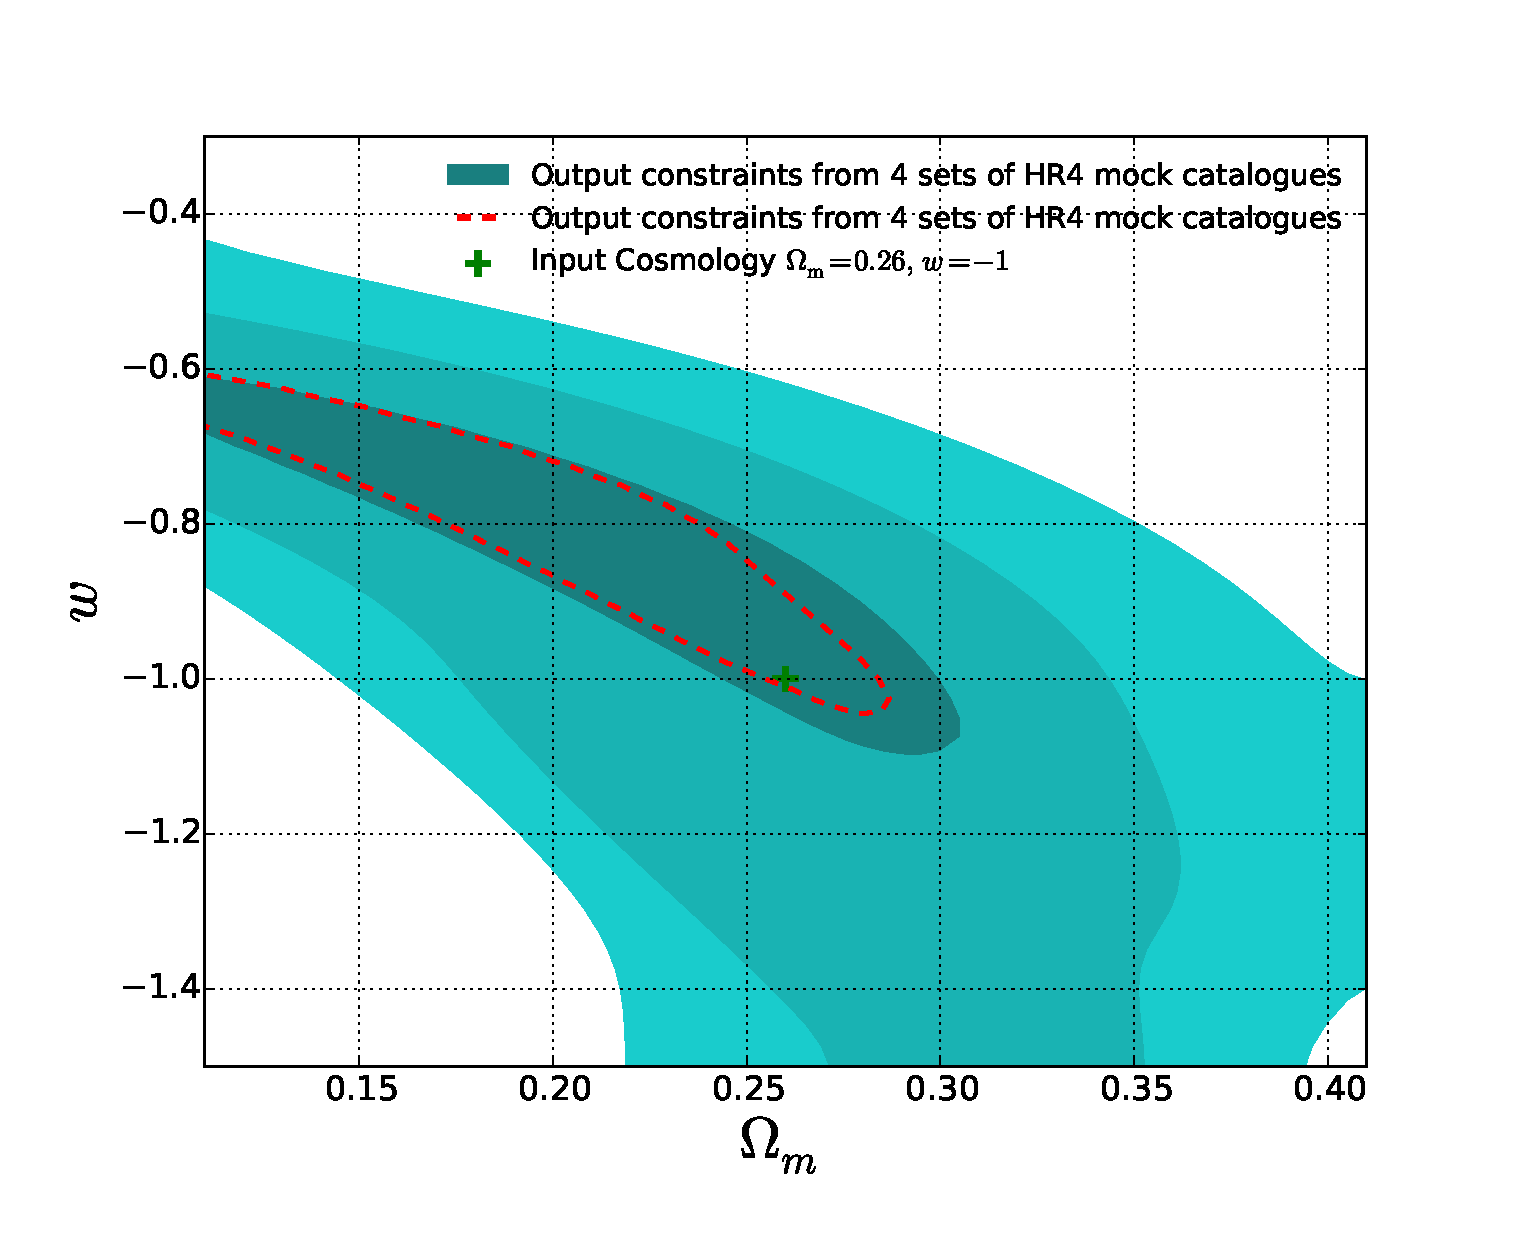
\includegraphics[width=6cm]{figIO.eps}
   %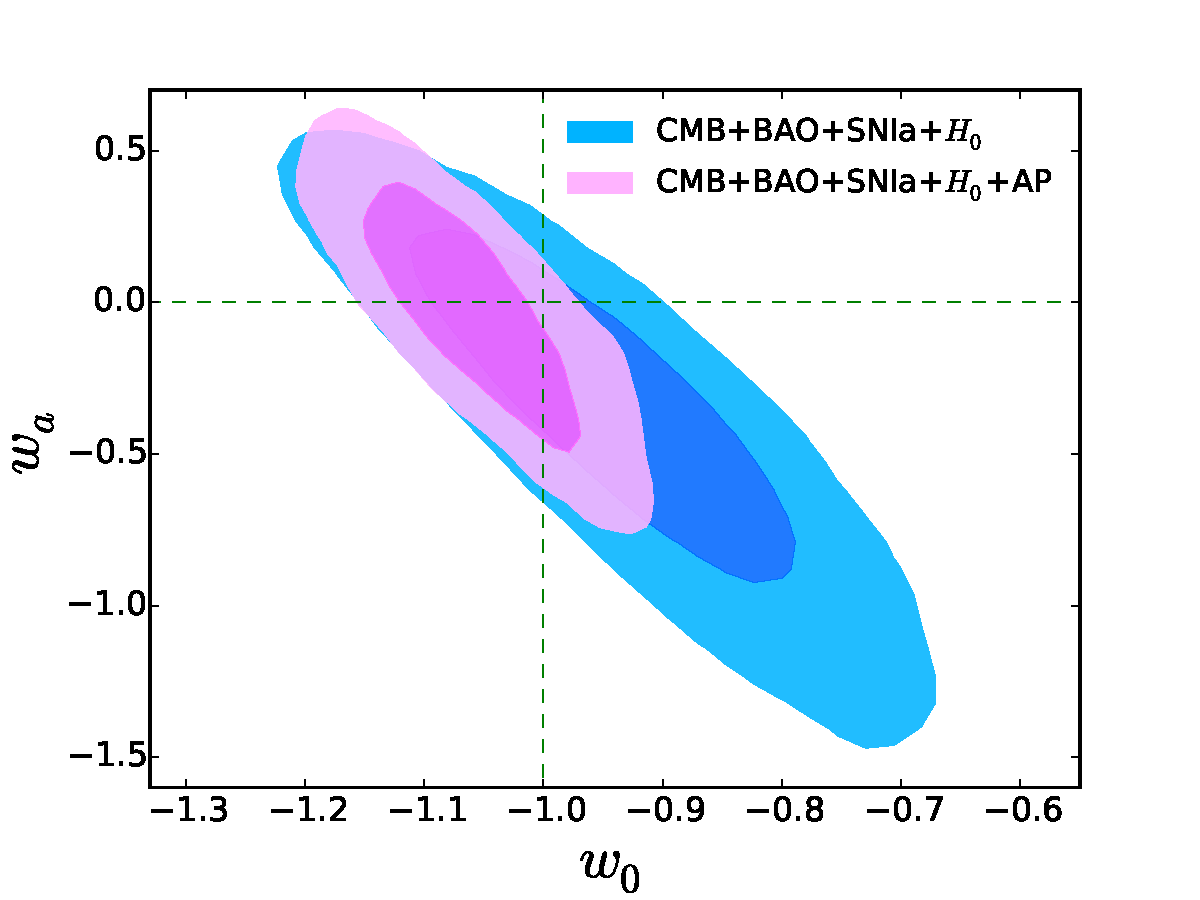
\includegraphics[width=9cm,natwidth=4,natheight=4]{fig2b.pdf}
   %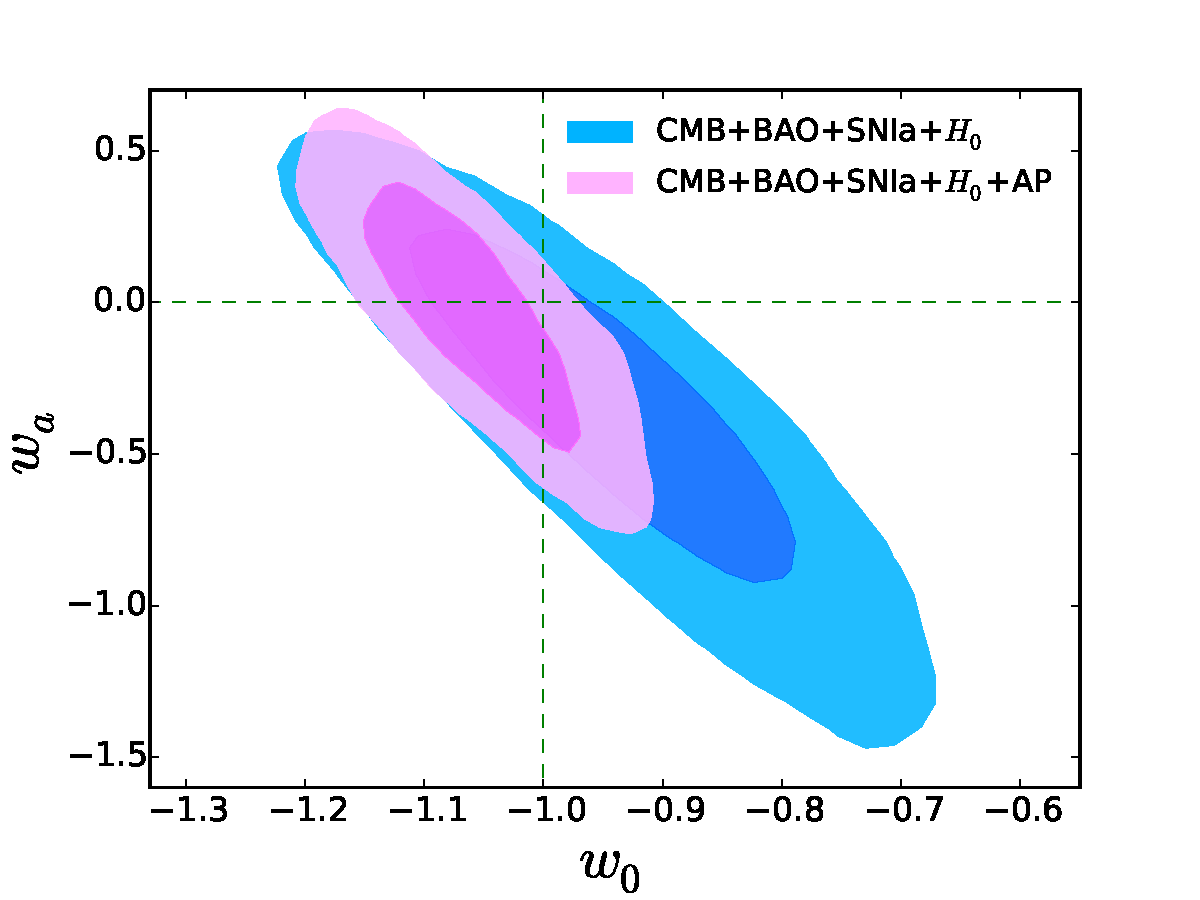
\includegraphics[height=8cm]{fig2b.pdf}
%   \includegraphics[height=8cm]{Tpcf--plot--Normed.eps}
%    \includegraphics[height=8cm]{smu.eps}
   }
   \caption{\label{fig_IO}
   Input-output test of our method.
   }
\end{figure*}



\section{Reproducing wCDM Constraints}

We firstly try to reproduce the constraints on $\Omega_m$ and $w$ in \citep{Li2016}:
\begin{equation}\label{eq:wcdm_constrain_default}
 \Omega_m=0.301\pm 0.006, w=−1.054\pm 0.025.
\end{equation}
Using the technique of approximate 2pCF and taking a fiducial of $\Omega_m=0.26, w=-1$, we obtains
\begin{equation}
\Omega_m = 0.301 \pm 0.008,\ w=-1.053\pm 0.034\ (\rm fid:\ \Omega_m=0.26, w=-1.0).
%    1  0.3010870E+00  0.7818562E-02  0.2973018E+00  0.3045011E+00  0.2883318E+00  0.3150334E+00   \Omega_m
%    2  0.6886453E+00  0.8507156E-02  0.6802557E+00  0.6975813E+00  0.6708444E+00  0.7047652E+00   h
%    3 -0.1053343E+01  0.3395215E-01 -0.1087474E+01 -0.1020395E+01 -0.1121890E+01 -0.9819443E+00   w
\end{equation}
while taking a different fiducial cosmology yields
\begin{eqnarray}
\Omega_m = 0.300 \pm 0.008,\ w=-1.057\pm 0.034\ (\rm fid:\ \Omega_m=0.26, w=-0.6),\\    
%param  mean           sddev          lower1         upper1         lower2         upper2         
%    1  0.3000053E+00  0.7703564E-02  0.2956289E+00  0.3032603E+00  0.2886989E+00  0.3142216E+00   \Omega_m
%   2  0.6898875E+00  0.8383848E-02  0.6805430E+00  0.6979808E+00  0.6721509E+00  0.7035974E+00   h
%    3 -0.1057455E+01  0.3363486E-01 -0.1090917E+01 -0.1020533E+01 -0.1116405E+01 -0.9873376E+00   w
%\Omega_m = 0.304 \pm 0.007,\ w=-1.040\pm 0.030\ (\Omega_m=0.26, w=-1.4),\\
%    1  0.3037843E+00  0.7243439E-02  0.3005621E+00  0.3073846E+00  0.2911318E+00  0.3154794E+00   \Omega_m
%    2  0.6852584E+00  0.7600452E-02  0.6780053E+00  0.6935965E+00  0.6714114E+00  0.7010620E+00   h
%    3 -0.1040019E+01  0.3026509E-01 -0.1069579E+01 -0.1011192E+01 -0.1105126E+01 -0.9823171E+00   w
\Omega_m = 0.301 \pm 0.009,\ w=-1.055\pm 0.039\ (\rm fid:\ \Omega_m=0.31, w=-1.0),\\
%1  0.3007960E+00  0.8740571E-02  0.2960415E+00  0.3046011E+00  0.2873819E+00  0.3166509E+00   \Omega_m
    %2  0.6890261E+00  0.9820733E-02  0.6785434E+00  0.6990516E+00  0.6684322E+00  0.7058833E+00   h
    %3 -0.1054663E+01  0.3932623E-01 -0.1094898E+01 -0.1014076E+01 -0.1125992E+01 -0.9715273E+00   w
\Omega_m = 0.302 \pm 0.008,\ w=-1.050\pm 0.035\ (\rm fid:\ \Omega_m=0.31, w=-0.6),\\    
%    1  0.3015603E+00  0.8075695E-02  0.2970461E+00  0.3054528E+00  0.2890849E+00  0.3157329E+00   \Omega_m
%    2  0.6879760E+00  0.8903611E-02  0.6783486E+00  0.6972412E+00  0.6704429E+00  0.7035974E+00   h
%    3 -0.1050127E+01  0.3579852E-01 -0.1087200E+01 -0.1012397E+01 -0.1116100E+01 -0.9792085E+00   w
\Omega_m = 0.301 \pm 0.009,\ w=-1.052\pm 0.038\ (\rm fid:\ \Omega_m=0.31, w=-1.4),\\    
%    1  0.3010573E+00  0.8626961E-02  0.2960266E+00  0.3049617E+00  0.2883365E+00  0.3169329E+00   \Omega_m
%    2  0.6886086E+00  0.9597560E-02  0.6785247E+00  0.6981217E+00  0.6679604E+00  0.7046714E+00   h
%    3 -0.1052455E+01  0.3836365E-01 -0.1091669E+01 -0.1013558E+01 -0.1123257E+01 -0.9702918E+00   w
\Omega_m = 0.304 \pm 0.008,\ w=-1.037\pm 0.034\ (\rm fid:\ \Omega_m=0.11, w=-2.0).\\    
%    1  0.3042033E+00  0.7885861E-02  0.2999004E+00  0.3075644E+00  0.2920431E+00  0.3184511E+00   \Omega_m
%    2  0.6846982E+00  0.8425114E-02  0.6751794E+00  0.6930507E+00  0.6671152E+00  0.6988545E+00   h
%    3 -0.1037306E+01  0.3351825E-01 -0.1069483E+01 -0.1000567E+01 -0.1095984E+01 -0.9663453E+00   w
% 
\end{eqnarray}
so the derived constraints are rather insensitive to the fiducial cosmology.
Even the extremely wrong fiducial cosmology $\Omega_m=0.11, w=-2.0$ yields correct estimation of parameters.

We will use two fiducial cosmologies,
the $\Omega_m=0.26,\ 0.31$ $\Lambda$CDM models which are the best-fit cosmologies of WMAP5 \cite{WMAP5} and \cite{Planck}.
Averaging the 2pCFs inferred from the two fiducial cosmologies we get
\begin{equation}
\Omega_m = 0.301 \pm 0.008,\ w=-1.054\pm 0.036.
%    1  0.2991453E+00  0.7662944E-02  0.2951697E+00  0.3023594E+00  0.2871742E+00  0.3130522E+00   \Omega_m
%    2  0.6910298E+00  0.8322516E-02  0.6830850E+00  0.6999792E+00  0.6728376E+00  0.7055694E+00   h
%    3 -0.1062378E+01  0.3310274E-01 -0.1097275E+01 -0.1030780E+01 -0.1125694E+01 -0.9921285E+00   w
\end{equation}
The constraints are well consistent with Equation \ref{eq:wcdm_constrain_default},
except a slightly larger error bar due to the limitation of approximation method
\footnote{Equation \ref{eq:wcdm_constrain_default} was derived using $n_{\mu}$=25-35.
Using the approximate 2pCF the contour becomes noisy if using such a large number of $n_\mu$,
so we adopts $n_\mu$=20-25 for consideration of safty, although the derived constraints on $\Omega_m$ and $w$ are still consistent with 
Equation \ref{eq:wcdm_constrain_default}.
%%For constraints from the approximate 2pCF we use $n_{\mu}$=20-25.
%We could get a tighter constraint with similar means values of $\Omega_m$ and $w$ by using larger $n_\mu$.
%However, due to the limited accuray of the approximation, the contour becomes noisy if $n_\mu$ is larger.
%So we use $n_\mu<25$ for a consideration of safty. 
}.
%from the 
%The approximate 2pCF may not be accurate enough }


%Using other fiducial cosmologies we derive similar cosmological constraints...
%We simply adopt the $\Omega_m=0.26, w=-1$ as the fiducial cosmology in the following analysis...

\section{Input-Output Test}

We did an input-output test on four realizations of HR4 mocks \cite{hr4}.
Figure \ref{fig_IO} shows the input cosmology (marker by green plus) is recovered at $\sim$0.5$\sigma$.
I.e., it is recovered at $\sim$1$\sigma$ in case of using 1 realisation.

\begin{figure*}
   \centering{
   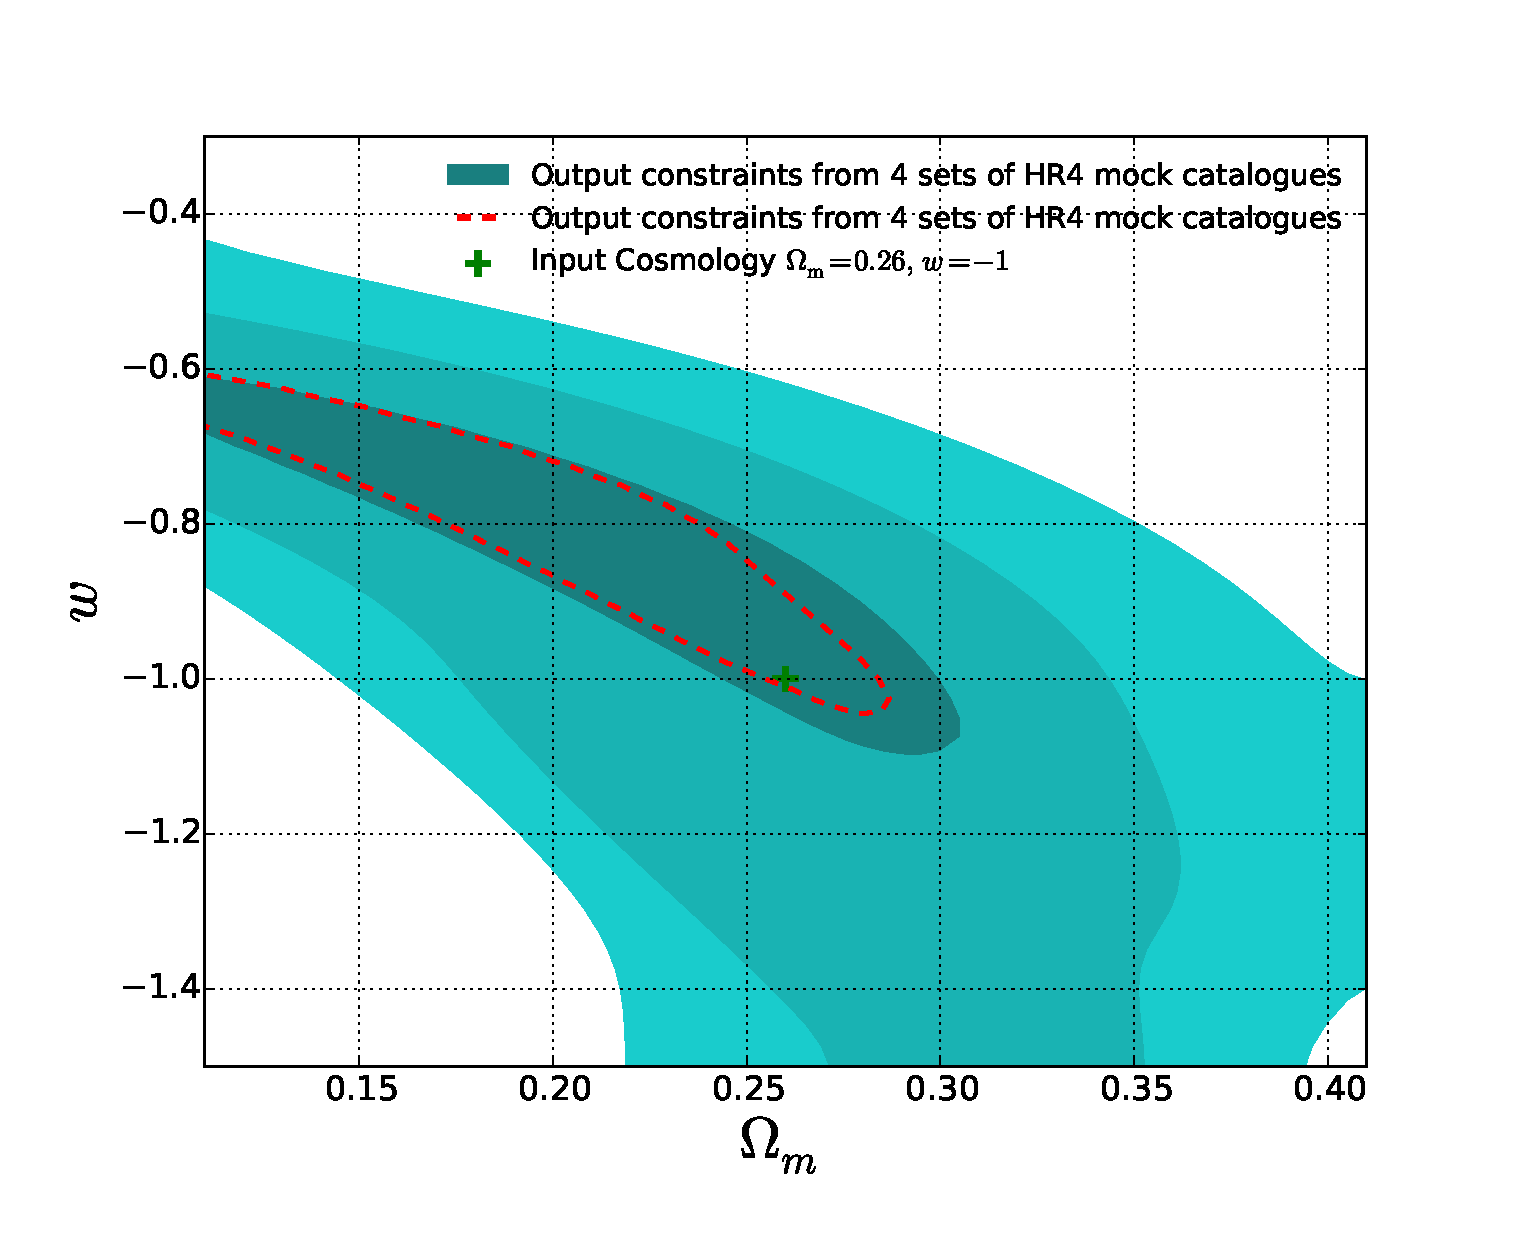
\includegraphics[width=6cm]{figIO.eps}
   %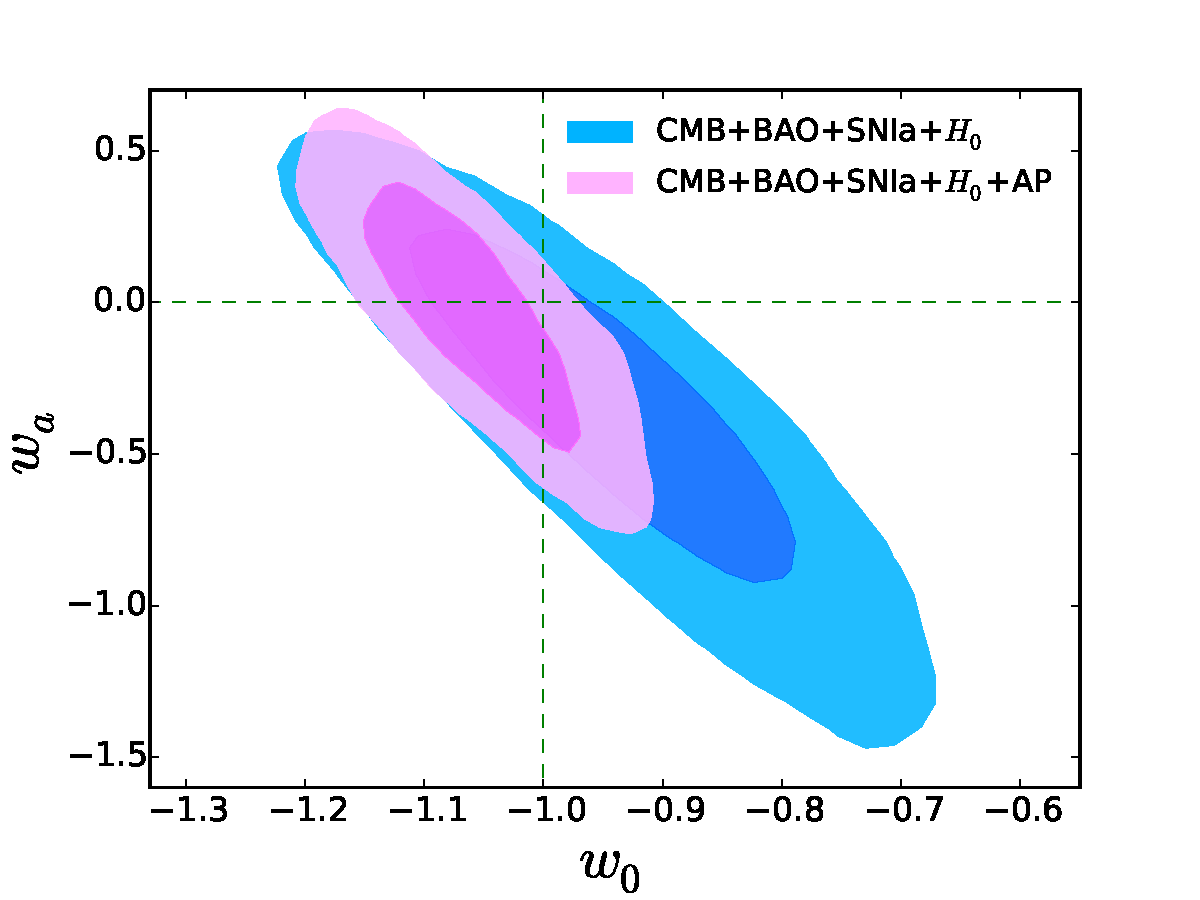
\includegraphics[width=9cm,natwidth=4,natheight=4]{fig2b.pdf}
   %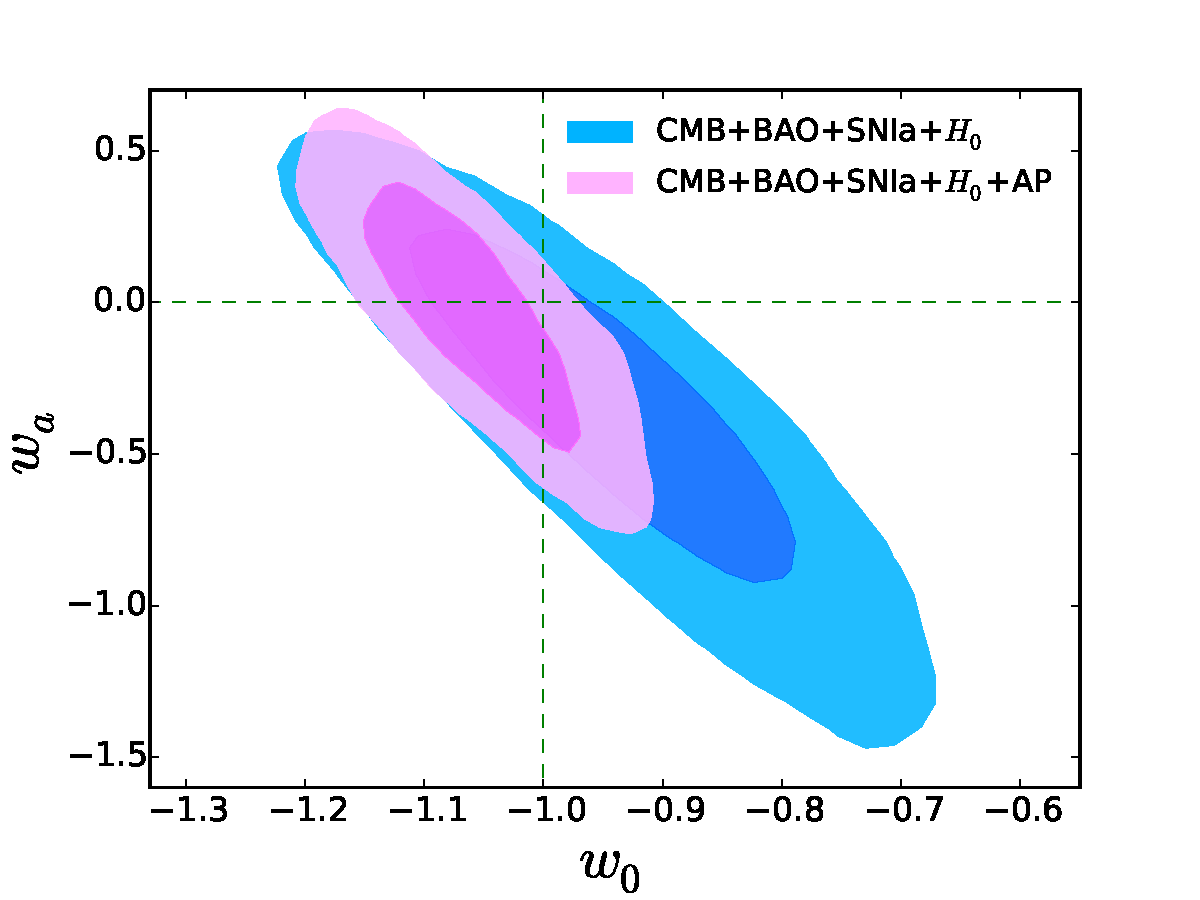
\includegraphics[height=8cm]{fig2b.pdf}
%   \includegraphics[height=8cm]{Tpcf--plot--Normed.eps}
%    \includegraphics[height=8cm]{smu.eps}
   }
   \caption{\label{fig_IO}
   Input-output test of our method.
   }
\end{figure*}

\section{Constraints on CPL}


Combining our method with CMB+BAO+JLA+$H_0$ we derive the following constraints on CPL parameters
\begin{equation}
%\Omega_m = 0.300 \pm 0.008, w_0 = -1.056 \pm 0.061, w_a = -0.04 \pm 0.27,
    %1  0.2999656E+00  0.7616334E-02  0.2958745E+00  0.3035033E+00  0.2878169E+00  0.3132870E+00   \Omega_m
    %2  0.6904801E+00  0.8675444E-02  0.6808558E+00  0.6993898E+00  0.6722945E+00  0.7052207E+00   h
    %3 -0.1056468E+01  0.6096323E-01 -0.1116874E+01 -0.9965903E+00 -0.1175041E+01 -0.9287388E+00   w
    %4 -0.3808376E-01  0.2716607E+00 -0.3105235E+00  0.2321461E+00 -0.6033103E+00  0.4782076E+00   w_a    
\Omega_m = 0.301 \pm 0.008, w_0 = -1.042 \pm 0.067, w_a = -0.07 \pm 0.29,    
%    1  0.3014353E+00  0.7759923E-02  0.2974325E+00  0.3048882E+00  0.2889838E+00  0.3152269E+00   \Omega_m
%    2  0.6887652E+00  0.8760036E-02  0.6797134E+00  0.6978279E+00  0.6703971E+00  0.7044224E+00   h
%    3 -0.1041626E+01  0.6732817E-01 -0.1107730E+01 -0.9768319E+00 -0.1172149E+01 -0.8979017E+00   w
%    4 -0.7173374E-01  0.2860547E+00 -0.3572176E+00  0.2107347E+00 -0.6775045E+00  0.4558817E+00   w_a    
\end{equation}
whose error bars are $~30-40\%$ smaller than the result without adding our method
\begin{equation}
\Omega_m = 0.309 \pm 0.010, w_0 = -0.938 \pm 0.109, w_a = -0.38 \pm 0.41.
%    1  0.3086006E+00  0.9639142E-02  0.3039045E+00  0.3131096E+00  0.2926126E+00  0.3249674E+00   \Omega_m
%    2  0.6809952E+00  0.1054577E-01  0.6703974E+00  0.6916269E+00  0.6605231E+00  0.7026640E+00   h
%    3 -0.9377990E+00  0.1092489E+00 -0.1046659E+01 -0.8303874E+00 -0.1149980E+01 -0.7142246E+00   w
%    4 -0.3777249E+00  0.4069512E+00 -0.7694896E+00  0.1941066E-01 -0.1285417E+01  0.3473089E+00   w_a
\end{equation}
Contour area is only 49\% of the size without adding our method.

The result is robust against options of the method:
(The following result are using code with bug; error bars slightly underestimated; 
but still make sense )
\begin{eqnarray}
 \Omega_m = 0.300 \pm 0.008, w_0 = -1.056 \pm 0.061, w_a = -0.04 \pm 0.27;\ (default)\\
    %1  0.2999656E+00  0.7616334E-02  0.2958745E+00  0.3035033E+00  0.2878169E+00  0.3132870E+00   \Omega_m
    %2  0.6904801E+00  0.8675444E-02  0.6808558E+00  0.6993898E+00  0.6722945E+00  0.7052207E+00   h
    %3 -0.1056468E+01  0.6096323E-01 -0.1116874E+01 -0.9965903E+00 -0.1175041E+01 -0.9287388E+00   w
    %4 -0.3808376E-01  0.2716607E+00 -0.3105235E+00  0.2321461E+00 -0.6033103E+00  0.4782076E+00   w_a    
 \Omega_m = 0.304 \pm 0.008, w_0 = -1.086 \pm 0.059, w_a = -0.17 \pm 0.24;\ (no\ sys\ correction)\\
%    1  0.3044516E+00  0.7617671E-02  0.3010136E+00  0.3081013E+00  0.2914476E+00  0.3173381E+00   \Omega_m
%    2  0.6843483E+00  0.8617640E-02  0.6761587E+00  0.6938366E+00  0.6685808E+00  0.7021433E+00   h
%    3 -0.1086432E+01  0.5887451E-01 -0.1142671E+01 -0.1030551E+01 -0.1202939E+01 -0.9582690E+00   w
%    4  0.1765419E+00  0.2459850E+00 -0.6998082E-01  0.4178197E+00 -0.3467499E+00  0.6369699E+00   w_a
 \Omega_m = 0.311 \pm 0.012, w_0 = -0.890 \pm 0.112, w_a = -0.54 \pm 0.37;\ (s_{min}=5)\\
%     1  0.3106795E+00  0.1247425E-01  0.3020454E+00  0.3193043E+00  0.2915571E+00  0.3297243E+00   \Omega_m
%    2  0.6790295E+00  0.1404107E-01  0.6636639E+00  0.6949009E+00  0.6570693E+00  0.7024209E+00   h
%    3 -0.8899288E+00  0.1124836E+00 -0.1012331E+01 -0.7776258E+00 -0.1120599E+01 -0.6979795E+00   w
%    4 -0.5414805E+00  0.3701807E+00 -0.8797662E+00 -0.1862461E+00 -0.1357982E+01  0.1905846E+00   w_a
 \Omega_m = 0.294 \pm 0.006, w_0 = -1.187 \pm 0.071, w_a = +0.36 \pm 0.25;\ (s_{min}=7)\\
%    1  0.2938521E+00  0.6158528E-02  0.2911826E+00  0.2957586E+00  0.2842091E+00  0.3060188E+00   \Omega_m
%    2  0.6975137E+00  0.7042138E-02  0.6914995E+00  0.7038382E+00  0.6796758E+00  0.7088302E+00   h
%    3 -0.1186888E+01  0.7087103E-01 -0.1261200E+01 -0.1119832E+01 -0.1329742E+01 -0.1047623E+01   w
%    4  0.3660142E+00  0.2524543E+00  0.1158432E+00  0.6578174E+00 -0.1460920E+00  0.8598785E+00   w_a
 \Omega_m = 0.294 \pm 0.011, w_0 = -1.190 \pm 0.121, w_a = +0.39 \pm 0.33;\ (s_{min}=7,\ n_{bin}=10-20)\\
%    1  0.2937945E+00  0.1118874E-01  0.2870627E+00  0.2950019E+00  0.2797860E+00  0.3202182E+00   \Omega_m
%    2  0.6976098E+00  0.1298396E-01  0.6862239E+00  0.7081303E+00  0.6632705E+00  0.7171370E+00   h
%    3 -0.1190472E+01  0.1214532E+00 -0.1295471E+01 -0.1068587E+01 -0.1343450E+01 -0.8785172E+00   w
%    4  0.3867600E+00  0.3289572E+00  0.5316268E-01  0.7079318E+00 -0.4221970E+00  0.8678967E+00   w_a
\Omega_m = 0.296 \pm 0.008, w_0 = -1.104 \pm 0.074, w_a = +0.84 \pm 0.27;\ (s_{min}=8)\\
%    1  0.2963656E+00  0.8091846E-02  0.2921788E+00  0.2984683E+00  0.2853060E+00  0.3124503E+00   \Omega_m
%    2  0.6948693E+00  0.9173349E-02  0.6855760E+00  0.7027217E+00  0.6701427E+00  0.7069792E+00   h
%    3 -0.1104197E+01  0.7402831E-01 -0.1171962E+01 -0.1041108E+01 -0.1237853E+01 -0.9225305E+00   w
%    4  0.8445697E-01  0.2694499E+00 -0.1750832E+00  0.3481107E+00 -0.4825598E+00  0.6305552E+00   w_a
\Omega_m = 0.304 \pm 0.010, w_0 = -1.040 \pm 0.092, w_a = -0.17 \pm 0.30;\ (s_{min}=8,\ n_{bin}=15-20)\\
%    1  0.3045034E+00  0.1005320E-01  0.2987972E+00  0.3086600E+00  0.2893736E+00  0.3229052E+00   \Omega_m
%    2  0.6850076E+00  0.1135499E-01  0.6718086E+00  0.6970528E+00  0.6625763E+00  0.7040868E+00   h
%    3 -0.1040081E+01  0.9299131E-01 -0.1123795E+01 -0.9480563E+00 -0.1207545E+01 -0.8285635E+00   w
%    4 -0.1743333E-01  0.3040112E+00 -0.3154785E+00  0.2747433E+00 -0.6685215E+00  0.5483677E+00   w_a
\Omega_m = 0.296 \pm 0.007, w_0 = -1.112 \pm 0.102, w_a = +0.14 \pm 0.31;\ (s_{min}=9)\\
%    1  0.2960495E+00  0.9065403E-02  0.2913228E+00  0.2979396E+00  0.2840257E+00  0.3162002E+00   \Omega_m
%    2  0.6952894E+00  0.1029523E-01  0.6850439E+00  0.7041332E+00  0.6678519E+00  0.7086220E+00   h
%    3 -0.1122218E+01  0.1023121E+00 -0.1206152E+01 -0.1040032E+01 -0.1301468E+01 -0.8461473E+00   w
%    4  0.1483019E+00  0.3109249E+00 -0.1317593E+00  0.4418245E+00 -0.5965950E+00  0.7171528E+00   w_a
\Omega_m = 0.292 \pm 0.005, w_0 = -1.214 \pm 0.061, w_a = +0.43 \pm 0.23;\ (s_{min}=10)\\
%    1  0.2917479E+00  0.4707289E-02  0.2900463E+00  0.2945549E+00  0.2838218E+00  0.2991014E+00   \Omega_m
%    2  0.7001461E+00  0.5035239E-02  0.6953868E+00  0.7051628E+00  0.6890005E+00  0.7093625E+00   h
%    3 -0.1214425E+01  0.6121805E-01 -0.1281762E+01 -0.1154465E+01 -0.1343450E+01 -0.1095344E+01   w
%    4  0.4321809E+00  0.2353314E+00  0.1999038E+00  0.7011163E+00 -0.4254742E-01  0.9881712E+00   w_a
\Omega_m = 0.293 \pm 0.004, w_0 = -1.244 \pm 0.067, w_a = +0.55 \pm 0.23;\ (s_{min}=15)\\
%    1  0.2926859E+00  0.4474665E-02  0.2908476E+00  0.2951106E+00  0.2856461E+00  0.2983049E+00   \Omega_m
%    2  0.6988735E+00  0.4830248E-02  0.6948004E+00  0.7034968E+00  0.6894865E+00  0.7065223E+00   h
%    3 -0.1243898E+01  0.6722018E-01 -0.1301468E+01 -0.1198655E+01 -0.1343450E+01 -0.1109980E+01   w
%    4  0.5542613E+00  0.2332418E+00  0.3651496E+00  0.7219638E+00  0.7491230E-01  0.9881712E+00   w_a
\Omega_m = 0.294 \pm 0.005, w_0 = -1.206 \pm 0.070, w_a = +0.45 \pm 0.25;\ (s_{min}=20)\\
%    1  0.2939366E+00  0.5389950E-02  0.2918451E+00  0.2958401E+00  0.2856461E+00  0.3038239E+00   \Omega_m
%    2  0.6968561E+00  0.6166073E-02  0.6916268E+00  0.7034390E+00  0.6826143E+00  0.7079047E+00   h
%    3 -0.1205723E+01  0.7032741E-01 -0.1262913E+01 -0.1137256E+01 -0.1301468E+01 -0.1021863E+01   w
%    4  0.4528745E+00  0.2538872E+00  0.2033804E+00  0.7079318E+00 -0.1364700E+00  0.8598785E+00   w_a
\Omega_m = 0.305 \pm 0.008, w_0 = -1.012 \pm 0.063, w_a = -0.12 \pm 0.27;\ (s_{max}=30)\\
%    1  0.3053987E+00  0.8052183E-02  0.3010878E+00  0.3093758E+00  0.2924301E+00  0.3189678E+00   \Omega_m
%    2  0.6839926E+00  0.9046344E-02  0.6740993E+00  0.6937786E+00  0.6673111E+00  0.7009633E+00   h
%    3 -0.1011791E+01  0.6292610E-01 -0.1073540E+01 -0.9492997E+00 -0.1131292E+01 -0.8786243E+00   w
%    4 -0.1152784E+00  0.2749302E+00 -0.3924667E+00  0.1655942E+00 -0.6961722E+00  0.3878639E+00   w_a
 \Omega_m = 0.300 \pm 0.008, w_0 = -1.070 \pm 0.067, w_a = -0.15 \pm 0.27;\ (s_{max}=50)\\
%    1  0.2998153E+00  0.8176648E-02  0.2951764E+00  0.3039279E+00  0.2866067E+00  0.3137714E+00   \Omega_m
%    2  0.6905681E+00  0.9393440E-02  0.6801617E+00  0.7005698E+00  0.6721556E+00  0.7066163E+00   h
%    3 -0.1069798E+01  0.6747674E-01 -0.1139699E+01 -0.1001953E+01 -0.1197799E+01 -0.9313961E+00   w
%    4  0.1513314E-01  0.2712663E+00 -0.2532490E+00  0.2766477E+00 -0.5694581E+00  0.5231100E+00   w_a
%\Omega_m = 0.300 \pm 0.076, w_0 = -1.056 \pm 0.061, w_a = -0.04 \pm 0.27;\ (default)\\ 
 \Omega_m = 0.301 \pm 0.008, w_0 = -1.042 \pm 0.067, w_a = -0.07 \pm 0.29;\ (fid:\ \Omega_m=0.26)\\
%    1  0.3014353E+00  0.7759923E-02  0.2974325E+00  0.3048882E+00  0.2889838E+00  0.3152269E+00   \Omega_m
%    2  0.6887652E+00  0.8760036E-02  0.6797134E+00  0.6978279E+00  0.6703971E+00  0.7044224E+00   h
%    3 -0.1041626E+01  0.6732817E-01 -0.1107730E+01 -0.9768319E+00 -0.1172149E+01 -0.8979017E+00   w
%    4 -0.7173374E-01  0.2860547E+00 -0.3572176E+00  0.2107347E+00 -0.6775045E+00  0.4558817E+00   w_
 \Omega_m = 0.302 \pm 0.009, w_0 = -1.031 \pm 0.111, w_a = -0.11 \pm 0.31;\ (fid:\ \Omega_m=0.31)\\
%    1  0.3019978E+00  0.9037630E-02  0.2968538E+00  0.3062673E+00  0.2879927E+00  0.3180927E+00   \Omega_m
%    2  0.6882447E+00  0.1022173E-01  0.6771768E+00  0.6989502E+00  0.6676515E+00  0.7056603E+00   h
%    3 -0.1030251E+01  0.8464437E-01 -0.1112791E+01 -0.9444134E+00 -0.1178093E+01 -0.8387510E+00   w
%    4 -0.1095804E+00  0.3116813E+00 -0.4190273E+00  0.2000228E+00 -0.7960000E+00  0.4415740E+00   w_a
\Omega_m = 0.301 \pm 0.008, w_0 = -1.027 \pm 0.076, w_a = -0.14 \pm 0.30;\ (fid:\ \Omega_m=0.31,\ w=-1.4)\\
%1  0.3011573E+00  0.8231730E-02  0.2965841E+00  0.3044093E+00  0.2889176E+00  0.3167123E+00   \Omega_m
%    2  0.6893068E+00  0.9233476E-02  0.6791262E+00  0.6980940E+00  0.6685460E+00  0.7040868E+00   h
%    3 -0.1026551E+01  0.7639796E-01 -0.1103179E+01 -0.9542612E+00 -0.1179271E+01 -0.8682009E+00   w
%    4 -0.1422300E+00  0.3023214E+00 -0.4418920E+00  0.1692683E+00 -0.7694896E+00  0.4188722E+00   w_a
\Omega_m = 0.302 \pm 0.008, w_0 = -1.028 \pm 0.074, w_a = -0.12 \pm 0.29;\ (fid:\ \Omega_m=0.31,\ w=-0.6)\\
%    1  0.3020827E+00  0.7924811E-02  0.2978336E+00  0.3057574E+00  0.2897049E+00  0.3161174E+00   \Omega_m
%    2  0.6880859E+00  0.8808431E-02  0.6786923E+00  0.6972611E+00  0.6703045E+00  0.7036877E+00   h
%    3 -0.1027672E+01  0.7365862E-01 -0.1101519E+01 -0.9552786E+00 -0.1167812E+01 -0.8736494E+00   w
%    4 -0.1166207E+00  0.2900048E+00 -0.4067305E+00  0.1745208E+00 -0.7335074E+00  0.4162662E+00   w_a
\Omega_m = 0.301 \pm 0.007, w_0 = -1.037 \pm 0.070, w_a = -0.10 \pm 0.29;\ (fid:\ \Omega_m=0.26,\ w=-0.6)\\
%    1  0.3006850E+00  0.7467012E-02  0.2966147E+00  0.3038277E+00  0.2893660E+00  0.3141890E+00   \Omega_m
%    2  0.6897466E+00  0.8230340E-02  0.6808848E+00  0.6978279E+00  0.6717161E+00  0.7035547E+00   h
%    3 -0.1037422E+01  0.7012652E-01 -0.1108159E+01 -0.9682866E+00 -0.1168990E+01 -0.8900837E+00   w
%    4 -0.1032858E+00  0.2868809E+00 -0.3892562E+00  0.1815807E+00 -0.7092019E+00  0.4296969E+00   w_a
\Omega_m = 0.303 \pm 0.007, w_0 = -1.02 \pm 0.066, w_a = -0.13 \pm 0.29;\ (fid:\ \Omega_m=0.26,\ w=-1.4)\\
%    1  0.3032544E+00  0.7414775E-02  0.2993517E+00  0.3069571E+00  0.2913482E+00  0.3158008E+00   \Omega_m
%    2  0.6866638E+00  0.8257572E-02  0.6782643E+00  0.6953868E+00  0.6710219E+00  0.7023747E+00   h
%    3 -0.1018870E+01  0.6596945E-01 -0.1081324E+01 -0.9556725E+00 -0.1148855E+01 -0.8798090E+00   w
%    4 -0.1312665E+00  0.2922572E+00 -0.4265570E+00  0.1617354E+00 -0.7551442E+00  0.3984255E+00   w_a
\Omega_m = 0.305 \pm 0.008, w_0 = -1.00 \pm 0.076, w_a = -0.18 \pm 0.31;\ (fid:\ \Omega_m=0.11,\ w=-2.0)\\
%    1  0.3046787E+00  0.8035600E-02  0.3003241E+00  0.3080979E+00  0.2924081E+00  0.3192678E+00   \Omega_m
%    2  0.6850740E+00  0.8883587E-02  0.6757190E+00  0.6938366E+00  0.6660933E+00  0.7010015E+00   h
%    3 -0.1001670E+01  0.7658665E-01 -0.1076535E+01 -0.9268110E+00 -0.1135934E+01 -0.8293599E+00   w
%    4 -0.1765842E+00  0.3140867E+00 -0.4861429E+00  0.1340849E+00 -0.8704449E+00  0.3855963E+00   w_a
 \Omega_m = 0.292 \pm 0.006, w_0 = -1.069 \pm 0.066, w_a = -0.16 \pm 0.26;\ (n_{\rm bin}=25-30)\\
%    1  0.2918158E+00  0.5628423E-02  0.2891825E+00  0.2941891E+00  0.2825581E+00  0.3010753E+00   \Omega_m
%    2  0.7010978E+00  0.5342961E-02  0.6965207E+00  0.7057875E+00  0.6904120E+00  0.7107044E+00   h
%    3 -0.1068860E+01  0.6574810E-01 -0.1135201E+01 -0.9997170E+00 -0.1192658E+01 -0.9359879E+00   w
%    4 -0.1599187E+00  0.2579696E+00 -0.4287996E+00  0.1009467E+00 -0.6869010E+00  0.3310719E+00   w_a 
 \Omega_m = 0.298 \pm 0.009, w_0 = -1.060 \pm 0.078, w_a = -0.06 \pm 0.28;\ (n_{\rm bin}=15-20)\\
%    1  0.2981509E+00  0.8480198E-02  0.2937075E+00  0.3010753E+00  0.2855200E+00  0.3145861E+00   \Omega_m
%    2  0.6929065E+00  0.9613244E-02  0.6833258E+00  0.7020276E+00  0.6693790E+00  0.7081825E+00   h
%    3 -0.1060092E+01  0.7841329E-01 -0.1137969E+01 -0.9868453E+00 -0.1204331E+01 -0.8823292E+00   w
%    4 -0.6177110E-01  0.2853058E+00 -0.3383224E+00  0.2207513E+00 -0.6736959E+00  0.4597655E+00   w_a
\Omega_m = 0.297 \pm 0.007, w_0 = -1.059 \pm 0.064, w_a = -0.09 \pm 0.29;\ (\mu_{\rm max}=0.99)\\
%    1  0.2970033E+00  0.7438703E-02  0.2932999E+00  0.3005298E+00  0.2844435E+00  0.3095693E+00   \Omega_m
%    2  0.6944156E+00  0.8562032E-02  0.6852347E+00  0.7034621E+00  0.6776627E+00  0.7097906E+00   h
%    3 -0.1059209E+01  0.6415386E-01 -0.1119685E+01 -0.9984353E+00 -0.1183662E+01 -0.9221239E+00   w
%    4 -0.9323390E-01  0.2891426E+00 -0.3791739E+00  0.1978428E+00 -0.7053933E+00  0.4386172E+00   w_a
\Omega_m = 0.297 \pm 0.008, w_0 = -1.049 \pm 0.067, w_a = -0.14 \pm 0.29;\ (\mu_{\rm max}=0.98)\\
%    1  0.2971641E+00  0.7942513E-02  0.2928890E+00  0.3007868E+00  0.2843925E+00  0.3111318E+00   \Omega_m
%    2  0.6943367E+00  0.9159705E-02  0.6838175E+00  0.7036877E+00  0.6756107E+00  0.7090616E+00   h
%    3 -0.1048832E+01  0.6735188E-01 -0.1115870E+01 -0.9809483E+00 -0.1178066E+01 -0.9137653E+00   w
%    4 -0.1356415E+00  0.2921079E+00 -0.4402006E+00  0.1614097E+00 -0.7334072E+00  0.4089997E+00   w_a
\Omega_m = 0.296 \pm 0.007, w_0 = -1.085 \pm 0.058, w_a = -0.03 \pm 0.26;\ (\mu_{\rm max}=0.95)\\
%    1  0.2958482E+00  0.6768659E-02  0.2925865E+00  0.2985238E+00  0.2851187E+00  0.3079769E+00   \Omega_m
%    2  0.6955895E+00  0.7603504E-02  0.6879188E+00  0.7027593E+00  0.6782961E+00  0.7083444E+00   h
%    3 -0.1085079E+01  0.5821141E-01 -0.1141841E+01 -0.1028412E+01 -0.1202939E+01 -0.9710419E+00   w
%    4 -0.2700702E-02  0.2556522E+00 -0.2484505E+00  0.2449754E+00 -0.5417479E+00  0.4950460E+00   w_a
\Omega_m = 0.295 \pm 0.009, w_0 = -1.042 \pm 0.078, w_a = -0.20 \pm 0.27;\ (\mu_{\rm max}=0.9)\\
%    1  0.2953501E+00  0.8772235E-02  0.2911129E+00  0.2967718E+00  0.2836995E+00  0.3152540E+00   \Omega_m
%    2  0.6967812E+00  0.1002391E-01  0.6893361E+00  0.7044224E+00  0.6687312E+00  0.7090616E+00   h
%    3 -0.1041509E+01  0.6787062E-01 -0.1105455E+01 -0.9768264E+00 -0.1164679E+01 -0.8928949E+00   w
%    4 -0.2046604E+00  0.2724470E+00 -0.4677980E+00  0.5854997E-01 -0.7367398E+00  0.3625436E+00   w_a
\Omega_m = 0.302 \pm 0.009, w_0 = -1.041 \pm 0.067, w_a = -0.07 \pm 0.33;\ (\mu_{\rm max}=0.85)\\
%    1  0.3019305E+00  0.8978132E-02  0.2964838E+00  0.3067806E+00  0.2881711E+00  0.3175436E+00   \Omega_m
%    2  0.6882045E+00  0.1060988E-01  0.6759042E+00  0.6993434E+00  0.6685460E+00  0.7051628E+00   h
%    3 -0.1040842E+01  0.6735301E-01 -0.1109551E+01 -0.9739134E+00 -0.1167705E+01 -0.9031411E+00   w
%    4 -0.7182715E-01  0.3319719E+00 -0.4230176E+00  0.2662489E+00 -0.7395587E+00  0.5367411E+00   w_a
\Omega_m = 0.300 \pm 0.008, w_0 = -1.060 \pm 0.061, w_a = -0.03 \pm 0.27;\ (1000\ mocks)\\
%    1  0.2996998E+00  0.7631856E-02  0.2955818E+00  0.3031793E+00  0.2876844E+00  0.3131096E+00   \Omega_m
%    2  0.6907899E+00  0.8691575E-02  0.6811798E+00  0.6996443E+00  0.6722945E+00  0.7054058E+00   h
%    3 -0.1060413E+01  0.6123963E-01 -0.1121439E+01 -0.1000457E+01 -0.1177598E+01 -0.9314673E+00   w
%    4 -0.2683176E-01  0.2692446E+00 -0.2932277E+00  0.2414674E+00 -0.5874053E+00  0.4886314E+00   w_a
\Omega_m = 0.301 \pm 0.009, w_0 = -1.036 \pm 0.066, w_a = -0.11 \pm 0.30;\ (no\ poly\ fit\ sys\ cor)\\
%    1  0.3009206E+00  0.8686461E-02  0.2958137E+00  0.3049704E+00  0.2878169E+00  0.3164586E+00   \Omega_m
%    2  0.6894864E+00  0.1008656E-01  0.6775701E+00  0.6995517E+00  0.6693154E+00  0.7052554E+00   h
%    3 -0.1035714E+01  0.6606381E-01 -0.1103748E+01 -0.9709249E+00 -0.1159458E+01 -0.9017237E+00   w
%    4 -0.1088647E+00  0.3011004E+00 -0.4243770E+00  0.2059112E+00 -0.7061951E+00  0.4541527E+00   w_a
\Omega_m = 0.304 \pm 0.007, w_0 = -1.064 \pm 0.064, w_a = +0.07 \pm 0.26;\ (No\ Last\ Bin)\\
%    1  0.3036060E+00  0.6765164E-02  0.3004900E+00  0.3068409E+00  0.2920387E+00  0.3148434E+00   \Omega_m
%    2  0.6856626E+00  0.7359859E-02  0.6786923E+00  0.6931423E+00  0.6716235E+00  0.7012467E+00   h
%    3 -0.1063599E+01  0.6351945E-01 -0.1123782E+01 -0.1003481E+01 -0.1181252E+01 -0.9185278E+00   w
%    4  0.6781013E-01  0.2590055E+00 -0.1836778E+00  0.3174407E+00 -0.5099973E+00  0.5439577E+00   w_a
% \Omega_m = 0.309 \pm 0.096, w_0 = -0.938 \pm 0.109, w_a = -0.38 \pm 0.41;\ ()\\
% \Omega_m = 0.309 \pm 0.096, w_0 = -0.938 \pm 0.109, w_a = -0.38 \pm 0.41;\ ()\\
% \Omega_m = 0.309 \pm 0.096, w_0 = -0.938 \pm 0.109, w_a = -0.38 \pm 0.41;\ ()\\
% \Omega_m = 0.309 \pm 0.096, w_0 = -0.938 \pm 0.109, w_a = -0.38 \pm 0.41;\ ()\\
% \Omega_m = 0.309 \pm 0.096, w_0 = -0.938 \pm 0.109, w_a = -0.38 \pm 0.41;\ ()\\
% \Omega_m = 0.309 \pm 0.096, w_0 = -0.938 \pm 0.109, w_a = -0.38 \pm 0.41;\ ()\\
\end{eqnarray}

%%% ### Average counts
%    1  0.3016429E+00  0.8317064E-02  0.2971790E+00  0.3053577E+00  0.2884946E+00  0.3165615E+00   \Omega_m
%    2  0.6885720E+00  0.9409753E-02  0.6786345E+00  0.6983718E+00  0.6690320E+00  0.7051628E+00   h
%    3 -0.1037858E+01  0.7408423E-01 -0.1109625E+01 -0.9662828E+00 -0.1176058E+01 -0.8741447E+00   w
%    4 -0.8379269E-01  0.2940539E+00 -0.3730223E+00  0.2081914E+00 -0.7163935E+00  0.4516133E+00   w_a
%%% ### Average counts


The result is fully consistent with a dark energy component having no evolution.
Adding the AP likelihood reduced the statistical errors by $\sim$40\%.
This demonstrate the power of the our method in constraining the redshift evolution of dark energy.

%0.290±0.053,  w=−1.07±0.15
%    1  0.3206192E+00  0.4302106E-01  0.2965672E+00  0.3494242E+00  0.2493646E+00  0.3805612E+00   \Omega_m
%    2  0.6975652E+00  0.5854719E-01  0.6279661E+00  0.7672566E+00  0.6044436E+00  0.7947755E+00   h
%    3 -0.1147537E+01  0.1289612E+00 -0.1276215E+01 -0.1017789E+01 -0.1422953E+01 -0.9082282E+00   w

%\subsection{Some Plottings, Discussions, Definition of $\chi^2$, ...}

%{\bf Figure: $\xi$ curves, in different cosmologies, without and with RSD}

\begin{figure*}
   \centering{
   %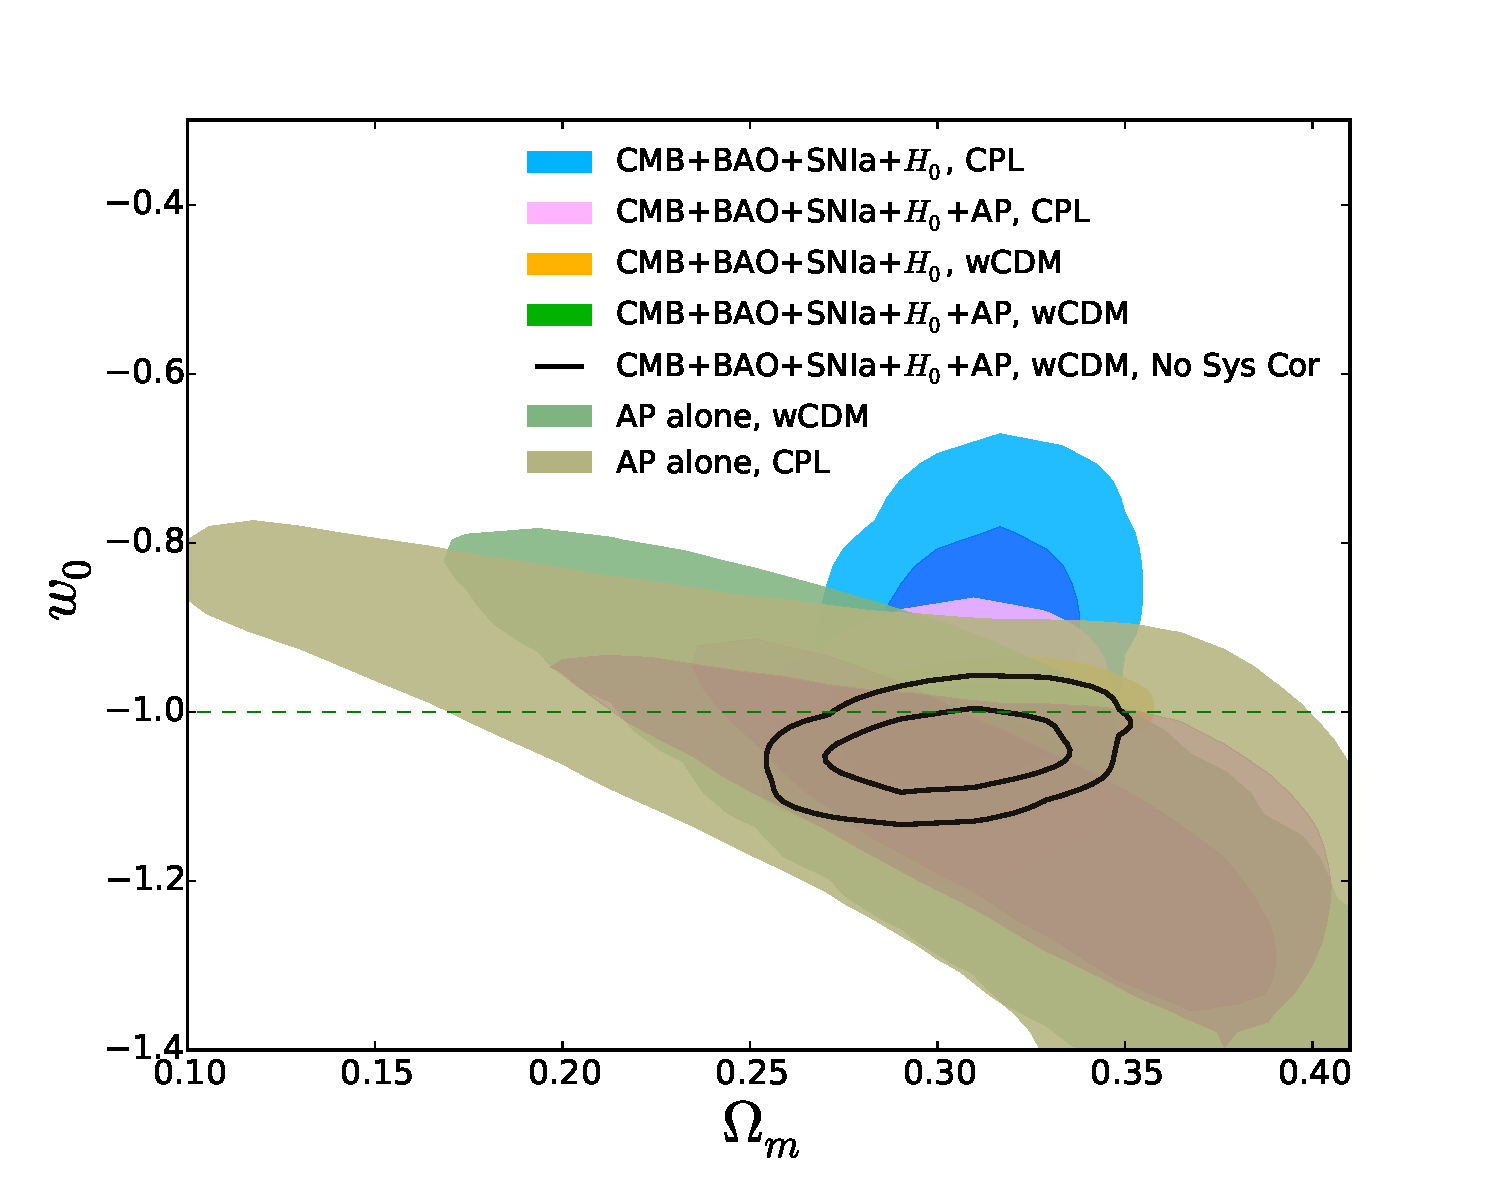
\includegraphics[width=9cm,natwidth=4,natheight=4]{figCPL_a.pdf}
   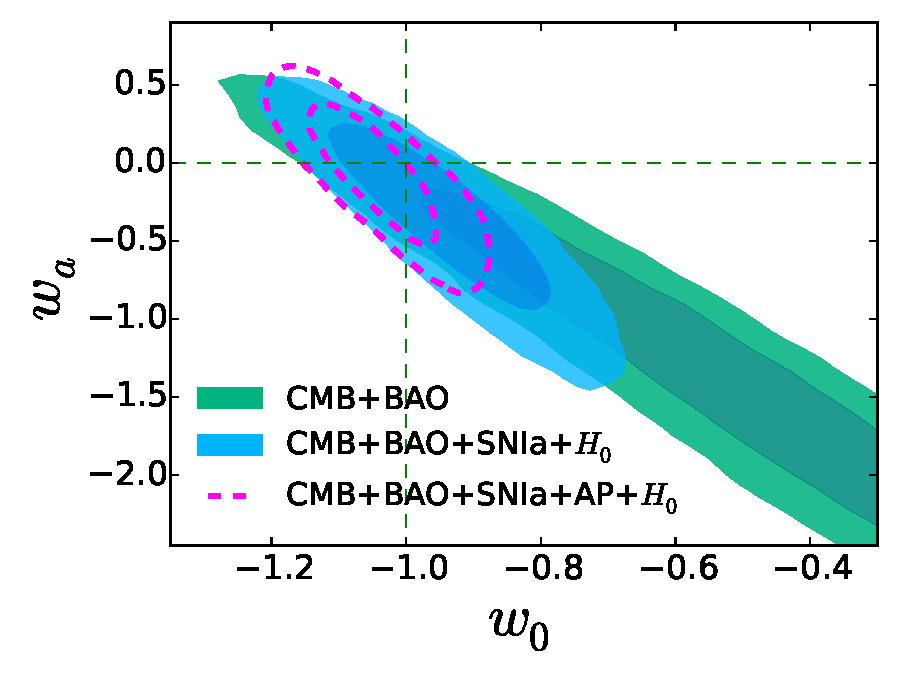
\includegraphics[width=7cm,natwidth=4,natheight=4]{figCPL_b.pdf}
   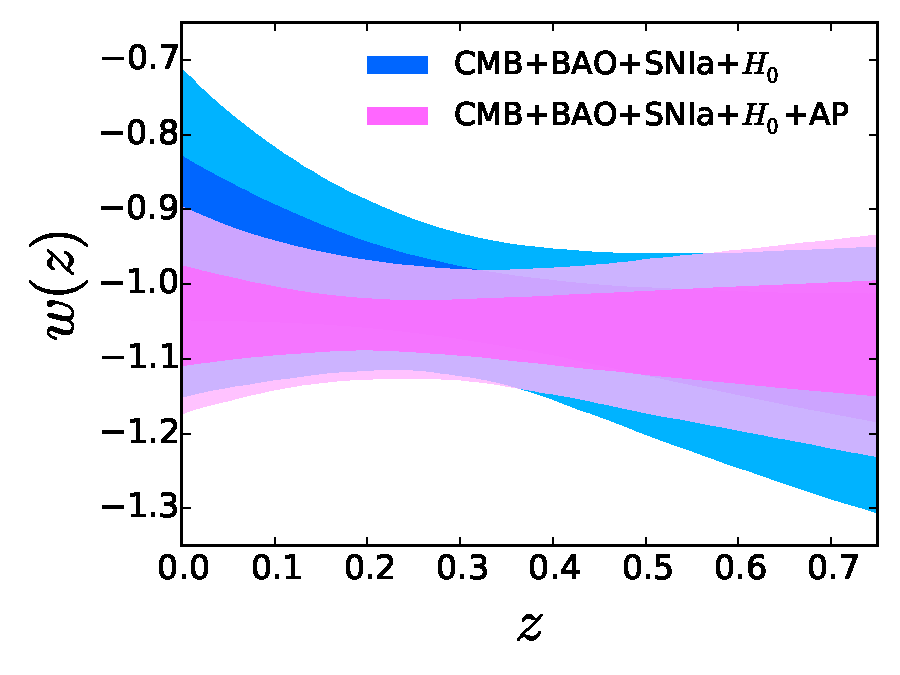
\includegraphics[width=7cm,natwidth=4,natheight=4]{figCPL_d.pdf}
   %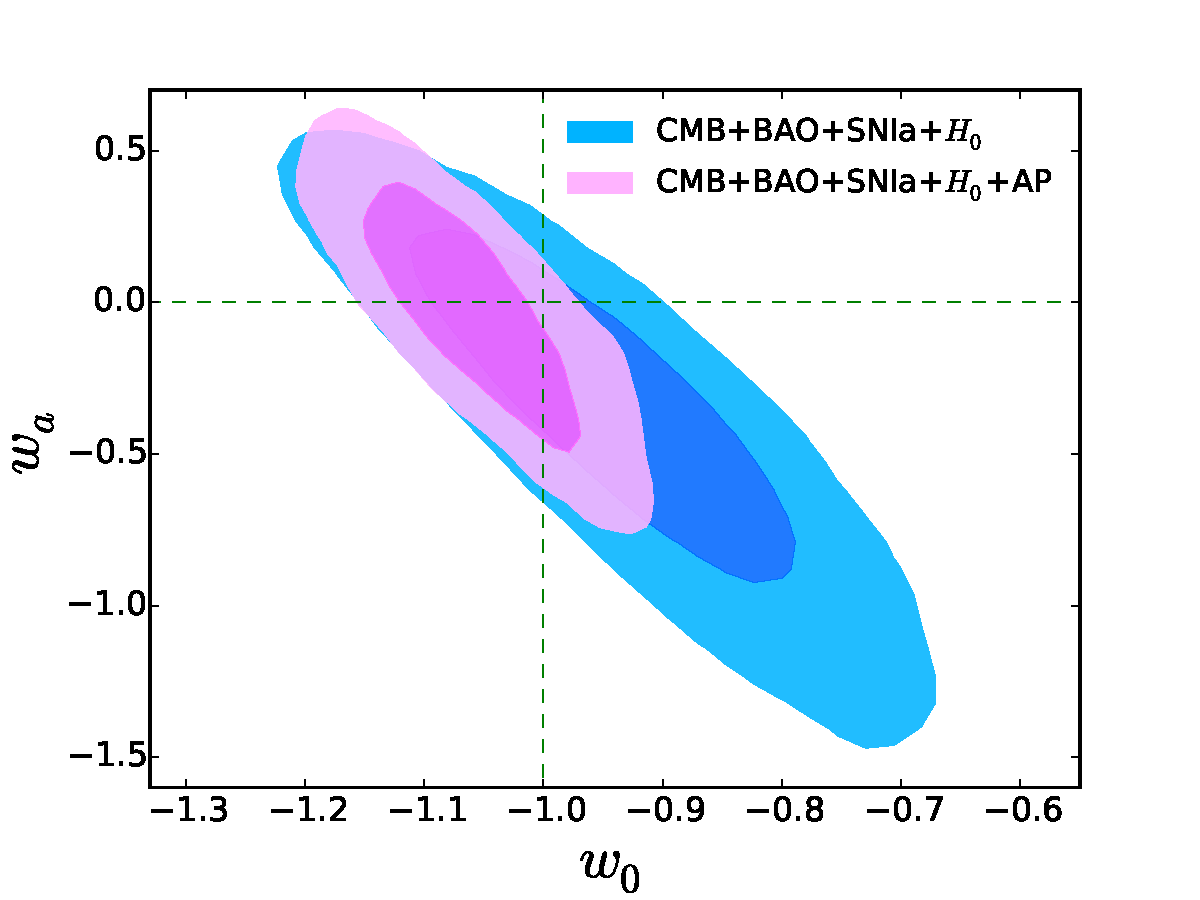
\includegraphics[height=8cm]{fig2b.pdf}
%   \includegraphics[height=8cm]{Tpcf--plot--Normed.eps}
%    \includegraphics[height=8cm]{smu.eps}
   }
   \caption{\label{fig_TpCF}
   Left panel: 68.3\%, 95.4\% CL likelihood contours in the $\Omega_m-w_0$ and $w_0-w_a$ plane.
   Results are consistent with $\Lambda$CDM.
   The constrained area is significantly reduced after adding the AP likelihood.
   This shows the power of the AP method in constraining dynamical dark energy.
   Right panel: Redshift evolution of $w(z)$, with/without adding AP method.
   Adding AP tightens the constraints and reduces the redshift evolution of $w$ (tilt of $w(z)$).
   }
\end{figure*}




\section*{Acknowledgments}

We thank the Korea Institute for Advanced Study for providing computing resources (KIAS Center for Advanced Computation Linux Cluster System).
We thank Seokcheon Lee and Graziano Rossi for many helpful discussions.


\begin{thebibliography}{}


\bibitem[Ade et al. (2015)]{Planck2015}
Ade, P.A.R., Aghanim, N., \& Arnaud, M., et al. arXiv:1502.01589

\bibitem[Alam et al.(2016)]{Alam2016}
Alam, S., Ata, M., \& Bailey, S., et al. 2016,
submitted to MNRAS (arXiv:1607.03155)

\bibitem[{{Alam} {et~al}\mbox{.}(2015{\natexlab{a}}){Alam}, {Albareti},
  {Allende Prieto}, {Anders}, {Anderson}, {Anderton}, {Andrews}, {Armengaud},
  {Aubourg}, {Bailey}, \& et~al.}]{dr12}
{Alam} S., Albareti, F.D.,\& Allende Prieto, C., {et~al.}, 2015,  ApJS, 219, 12

\bibitem[Alcock \& Paczynski(1979)]{AP1979}
Alcock, C., \& Paczynski, B. 1979, Nature, 281, 358  

%\bibitem[Anderson et al.(2012)]{2012MNRAS.427.3435A} 
%Anderson, L., Aubourg, E., Bailey, S., et al.\ 2012, MNRAS, 427, 3435

\bibitem[Anderson et al.(2013)]{Anderson2013}
Anderson, L., Aubourg, \'E., \& Bailey, S. et al. 2014, MNRAS, 441, 24  
  
%\bibitem[Bassett et al.(2002)]{Bassett2002}
%Bassett, B.A., Kunz, M., Silk, J., \& Ungarelli, C. 2002, MNRAS, 336, 1217

\bibitem[Ballinger, Peacock \& Heavens 1996]{Ballinger1996}
Ballinger, W.E., Peacock, J.A., \& Heavens, A.F. 1996, MNRAS, 282, 877  

\bibitem[Betoule et al.(2014)]{JLA}
Betoule, M., Kessler, R., \& Guy, J., et al. 2014, A\&A, 568, 32


\bibitem[Beutler et al.(2011)]{6dFGS}
Beutler, F., Blake, C., \& Colless, M., et al. 2011, MNRAS, 416, 3017

\bibitem[Beutler et al.(2013)]{Beutler2013}
Beutler, F., Saito, S., \& Seo, H.-J., et al. 2013, MNRAS, 443, 1065

\bibitem[Beutler et al.(2016)]{Beutler2016}
Beutler, F., Seo, H.-J., \& Saito, S., et al. 2016,
arXiv:1607.03150

\bibitem[Blake et al.(2011)]{Blake2011}
Blake, C., Glazebrook, K., \& Davis, T. M., 2011, MNRAS, 418, 1725  

\bibitem[Blake et al.(2013)]{WiggleZtopoloy}
Blake, C., James, J.B., \& Poole, G.B. 2013, MNRAS, 437, 2488

\bibitem[Bolton et al.(2012)]{Bolton2012}
Bolton, A.S., Schlegel, \& D.J., Aubourg E., et al. 2012, AJ, 144, 144

\bibitem[Boylan-Kolchin et al.(2008)]{B08}
Boylan-Kolchin, M., Ma, C.-P., \& Quataert, E. 2008, MNRAS, 383, 93


%\bibitem[Bueno Belloso et al. (2012)]{BB2012}
%Bueno Belloso, A., Pettinari, G.W., Meures, N., \& Percival, W.J. 2012, Phys. Rev. D, 86, 023530

%\bibitem[Chevallier \& Polarski(2001)]{CP2001}
%Chevallier, M., Polarski, D. 2001, Int. J. Mod. Phys. D, 10, 213


%\bibitem[Choi et al.(2010)]{choi 2010}
%Choi, Y.-Y., Park, C., Kim, J., Gott, J.R., 
%Weinberg, D.H., Vogeley, M.S., \& Kim, S.S. 2010, ApJS, 190, 181

\bibitem[Christensen et al.(2001)]{Bayesian}
Christensen, N., Meyer, R., Knox, L., \& Luey, B. 2001, Class. Quant. Grav., 18, 2677

%\bibitem[Chuang et al.(2013)]{Chuang2013}
%Chuang, C.-H., Prada, F., Beutler, F., et al. 2013, arXiv:1312.4889  

\bibitem[Chuang \& Wang(2012)]{ChuangWang2012}
Chuang, C.-H., \& Wang, Y. 2012, MNRAS, 426, 226  


%\bibitem[Corasaniti \& Copeland(2003)]{Corasaniti2003}
%Corasaniti, P.S., Copeland, E.J. 2003, Phys. Rev. D, 67, 063521

%eBOSS: 
%http://arxiv.org/abs/1508.04473
\bibitem[Dawson et al.(2015)]{eBOSS}
Dawson, K.S., Kneib, J.P., \& Percival, W.J., et al. 2015, accepted AJ

\bibitem[Dawson et al.(2012)]{Dawson et al. 2012}
Dawson, K.S., Schlegel, D.J., \& Ahn, C.P., et al. 2012, AJ, 145, 10

\bibitem[Efstathiou (2014)]{E14H0}
Efstathiou, G. 2014, MNRAS, 440, 1138

\bibitem[Eisenstein et al.(2011)]{Eisenstein et al. 2011}
Eisenstein, D.J.,  Weinberg, D.H., \& Agolet, E., et al. 2011, AJ, 142, 72

\bibitem[Feldman, Kaiser \& Peacock (1994)]{1994ApJ...426...23F} 
Feldman, H.A., Kaiser, N., \& Peacock, J.A.\ 1994, ApJ, 426, 23 

\bibitem[Fukugita et al. (1996)]{Fukugita1996}
Fukugita, M., Ichikawa, T., \& Gunn, J.E., et al. 1996, AJ, 111, 1748
%Publication:	
%Astronomical Journal v.111, p.1748 

%\bibitem[Gingold \& Monaghan(1977)]{GM1977}
%Gingold, R.A., \& Monaghan, J.J. 1977, MNRAS, 181, 375  

%\bibitem[Gott et al.(2009)]{gott 2009}
%Gott, J.R., Choi, Y.-Y., Park, C., \& Kim, J. 2009, ApJ, 695, L45  

%\bibitem[Gott et al.(2008)]{gott 2008}
%Gott, J.R., Hambrick, D.C., Vogeley, M.S., Kim, J., Park, C., Choi, Y.-Y.,
%Cen, R., Ostriker, J.P., \& Nagamine, K. 2008, ApJ, 675, 16  


\bibitem[Gunn et al. (1998)]{Gunn1998}	
Gunn, J.E., Carr, M., \& Rockosi, C. et al. 1998, AJ, 116, 3040

\bibitem[Gunn et al.(2006)]{Gunn et al. 2006}
Gunn, J.E., Siegmund, W.A., \& Mannery, E.J., et al. 2006, AJ, 131, 2332

\bibitem[Guzzo et al.(2008)]{Guzzo2008}
Guzzo, L., Pierleoni, M., \& Meneux, B., et al. 2008, Nature, 451, 541

\bibitem[Hartlap et al.(2006)]{Hartlap}
Hartlap J., Simon P. \& Schneider P. [astro-ph/0608064].


\bibitem[Hong et al.(2016)]{hong2016}
Hong, S.E., Park, C.,\&  Kim, J. 2016, ApJ, 823, 103

\bibitem[Jackson (1972)]{FOG}
Jackson, J., 1972, MNRAS, 156, 1

\bibitem[Jennings et al.(2011)]{Jennings2011}
Jennings, E., Baugh, C.M., \& Pascoli, S. 2011, MNRAS, 420, 1079  

%\bibitem[Jeong et al.(2014)]{Jeong2014}
%Jeong, D., Dai, L., Kamionkowski, M., \& Szalay, A.S. 2014, arXiv:1408.4648

\bibitem[Jiang et al.(2008)]{jiang2008}
Jiang, C.Y., Jing, Y. P., \& Faltenbacher, A., et al. 2008, ApJ, 675, 1095

\bibitem[Kaiser (1987)]{Kaiser1987}
Kaiser, N. 1987, MNRAS, 227, 1


\bibitem[Kim \& Park(2006)]{kim and park 2006}
Kim, J., \& Park, C. 2006, ApJ, 639, 600  

\bibitem[Kim et al.(2009)]{2009ApJ...701.1547K} 
Kim, J., Park, C., Gott, J.R., III, \& Dubinski, J.\ 2009, ApJ, 701, 1547 

\bibitem[Kim et al.(2015)]{hr4}
Kim, J., Park, C., L'Huillier, B., \& Hong, S. E. 2015, JKAS, 48, 213

\bibitem[Kim et al.(2011)]{horizonrun}
Kim, J., Park, C., Rossi, G., Lee, S.M., \& Gott, J.R. 2011, JKAS, 44, 217  

\bibitem[Kitaura et al.(2015)]{MDPATCHY}
Kitaura, F.S., Rodrı\'{i}guez-Torres, S., Chuang, C.-H., et al. arXiv:1509.06400

\bibitem[Komatsu et al.(2011)]{komatsu 2011}
Komatsu, E., Smith, K. M., \& Dunkley, J., et al. 2011, ApJS, 192, 18  

\bibitem[Lacey \& Cole(1993)]{LC93}
Lacey, C., \& Cole, S. 1993, MNRAS, 262, 627


\bibitem[Landy \& Szalay(1993)]{1993ApJ...412...64L} 
Landy, S.D., \& Szalay, A.S.\ 1993, ApJ, 412, 64 

%EUCLID:
%http://arxiv.org/abs/1110.3193
\bibitem[Laureijs et al.(2011)]{EUCLID}
Laureijs, R., Amiaux, J., \& Arduini, S., et al. 2011, arXiv:1110.3193

\bibitem[Lavaux \& Wandelt(2012)]{LavausWandelt1995}
Lavaux, G., \& Wandelt, B.D. 2012, ApJ, 754, 109  

%\bibitem[Levi et al.(2013)]{2013arXiv1308.0847L} 
%Levi, M., Bebek, C., Beers, T., et al.\ 2013, arXiv:1308.0847 

\bibitem[Lewis \& Bridle (2002)]{LB2002}
Lewis, A., \& Bridle, S. 2002, Phys. Rev. D, 66, 103511

\bibitem[L'Huillier et al.(2014)]{2014NewA...30...79L} 
L'Huillier, B., Park, C., \& Kim, J.\ 2014, New Astronomy, 30, 79 

\bibitem[Li et al.(2011)]{Li2011}
Li, M., Li, X.-D., Wang, S., \& Wang, Y. 2011, Commun. Theor. Phys., 56, 525

\bibitem[Li et al.(2014)]{Li2014}
Li, X.-D., Park, C., Forero-Romero, J., \& Kim, J. 2014, ApJ, 796, 137

\bibitem[Li et al.(2015)]{Li2015}
Li, X.-D., Park, C., Sabiu, C.G., \& Kim, J. 2015, MNRAS, 450, 807 

\bibitem[Li et al.(2015)]{Li2016}
Li, X.-D., Park, C., Sabiu, C.G., \& Kim, J. 2015, MNRAS, 450, 807 

%\bibitem[Linder(2003)]{Linder2003}
%Linder, E.V. 2003, Phys. Rev. Lett., 90, 091301

\bibitem[Linder et al.(2014)]{Linder2013}
Linder, E.V., Minji, O., Okumura, T., Sabiu, C.G., \& Song, Y.-S. 2014, Phys. Rev. D, 89, 063525  

\bibitem[L{\'o}pez-Corredoira(2014)]{2014ApJ...781...96L} 
L{\'o}pez-Corredoira, M.\ 2014, ApJ, 781, 96 

\bibitem[Mao et al. (2016)]{Qingqing2016}
Mao, Q., Berlind, A.A., Scherrer, R.J., et al. 2016, submitted to ApJ

\bibitem[Marinoni \& Buzzi(2010)]{Marinoni2010}
Marinoni, C., \& Buzzi, A. 2010, Nature, 468, 539  

\bibitem[Matsubara \& Suto(1996)]{Matsubara1996}
Matsubara T., \& Suto, Y. 1996, ApJ, 470, L1  

\bibitem[McCavana et al.(2012)]{M12}
McCavana, T., Micic, M., Lewis, G. F., et al. 2012, MNRAS, 424, 361


\bibitem[Morandi \& Sun (2016)]{MS2016}
Morandi, A., \& Sun, M. arXiv:1601.03741


\bibitem[Outram et al.(2004)]{Outram2004}
Outram, P.J., Shanks, T., Boyle, B.J., Croom, S.M., Hoyle, F., Loaring, N.S., 
Miller, L., \& Smith, R.J. 2004, MNRAS, 348, 745  

%\bibitem[Parejko et al.(2013)]{Parejko2013}
%Parejko, J. K., Sunayama, T., Padmanabhan, N., et al. 2013, MNRAS, 429, 98  

\bibitem[Parejko et al.(2013)]{Parejko2013}
Parejko J.K., et al., 2013, MNRAS, 429, 98

\bibitem[Parihar et al. (2014)]{CMASSLSS2014}
Parihar, P., Vogeley, M.S., \& Gott, J.R., et al. 2014, ApJ, 796, 86

\bibitem[Park et al.(2005)]{park 2005}
Park, C., Kim, J., \& Gott, J.R. 2005, ApJ, 633, 1  

\bibitem[Park \& Kim(2010)]{topology}
Park, C., \& Kim, Y.-R. 2010, ApJL, 715, L185  

\bibitem[Park et al. (2012)]{Park2012}
Park, C., Choi, Y.-Y., Kim, J., Gott, J.R., Kim, S.S., \&
Kim, K.-S. 2012, ApJ, 759, 7

\bibitem[Park et al. (2015)]{Park2015}
Park, C., Song, H., Einasto, M., Lietzen, H., \&
Heinamaki, P. 2015, JKAS, 48, 75

\bibitem[Peebles \& Ratra(2003)]{PR2003}
Peebles, P.J.E., \& Ratra, B. 2003, Reviews of Modern Physics, 75, 559

\bibitem[Percival et al.(2014)]{Percival2014}
Percival, W.J., Ross, A.J., \& S\'{a}nchez, A.G., et al. 2014, MNRAS, 439, 2531

\bibitem[Perlmutter et al.(1999)]{Perl1999}
Perlmutter, S., Aldering, G., \& Goldhaber, G., et al. 1999, ApJ, 517, 565  

\bibitem[Press \& Shechter(1974)]{PS1974}
Press, W.H., \& Schechter, P.L. 1974, ApJ, 187, 425



\bibitem[Reid et al.(2012)]{Reid2012}
Reid, B., Samushia, L., \& White, M., et al. 2012, MNRAS, 426, 2719  

\bibitem[Reid et al.(2016)]{Reidetal:2016}
Reid, B., Ho, S., \& Padmanabhan, N., et al.  2016, MNRAS, 455, 1553

\bibitem[Riess et al.(1998)]{Riess1998}
Riess, A.G., Filippenko, A.V., \& Challis, P., et al. 1998, AJ, 116, 1009  

\bibitem[Riess et al.(2011)]{Riess2011}
Riess, A.G., Macri, L., \& Casertano, S., et al. 2011, ApJ, 730, 119
%A 3\% Solution: Determination of the Hubble Constant with the Hubble Space Telescope and Wide Field Camera

\bibitem[Ross et al.(2012)]{2012MNRAS.424..564R} 
Ross, A.J., Percival, W.J., \& S{\'a}nchez, A.G. et al.\ 2012, MNRAS, 424, 564 

\bibitem[Ross et al.(2015)]{MGS}
Ross, A.J., Samushia, L., \& Howlett, C., et al. 2015, MNRAS, 449, 835

\bibitem[Ryden(1995)]{Ryden1995}
Ryden, B.S. 1995, ApJ, 452, 25  

%\bibitem[Samushia et al.(2014)]{Samushia2014}
%Samushia, L., Reid, B. A., White, M., et al. 2014, MNRAS, 439, 3504  

%\bibitem[Sanchez et al.(2013)]{Sanchez2013}
%Sanchez, A. G., Kazin, E. A., Beutler, F., et al. 2013, MNRAS, 433, 1202  

%\bibitem[Sutter et al.(2014)]{Sutter2014}
%Sutter, P.M., Pisani, A., Wandelt, B.D., \& Weinberg, D.H. 2014, MNRAS, 443, 2983


\bibitem[Sanchez et al.(2016)]{Sanchez2016}
Sanchez, A. G., Scoccimarro, R., \& Crocce, M., et al.
arXiv:1607.03147

\bibitem[Schlafly et al.(2010)]{Schlafly2010}
Schlafly E.F., Finkbeiner D.P., Schlegel D.J., et al. 2010, ApJ, 725, 1175

\bibitem[Schlafly \& Finkbeiner(2011)]{SF2011}
Schlafly E.F., \& Finkbeiner D.P. 2011, ApJ, 737, 103


%DESI:
%http://arxiv.org/abs/1106.1706
\bibitem[Schlegel et al.(2011)]{DESI}
Schlegel, D., Abdalla, F., \& Abraham, T., et al. 2011, arXiv:1106.1706

\bibitem[Smee et al.(2013)]{Smee2013}
Smee, S.A., Gunn, J.E., \& Uomoto, A., et al. 2013, AJ, 146, 32

\bibitem[Song et al.(2014)]{2014arXiv1407.2257S} 
Song, Y.S., Sabiu, C.G., 
Okumura, T., Oh, M., \& Linder, E.V.\ 2014, JCAP, 12, 005 

\bibitem[Speare et al. (2015)]{Speare2015}
Speare, R., Gott, J.R., Kim, J., \& Park, C.
2015, ApJ, 799, 176

%\bibitem[Tojeiro \& Percival(2011)]{Tojeiro2011}
%Tojeiro R., \& Percivial W.J. 2011, MNRAS, 417, 1114  

%\bibitem[Tojeiro et al.(2012)]{Tojeiro2012}
%Tojeiro, R., Percival, W. J., Wake, D. A., et al. 2012, MNRAS, 424, 136 

\bibitem[Viana \& Liddle(1996)]{VL1996}
Viana, P.T.P., \& Liddle, A.R. 1996, MNRAS, 281, 323

\bibitem[Villalobos et al.(2013)]{V13}
Villalobos, \'{A}., ́De Lucia, G., Weinmann, S.M., Borgani, S., \& Murante, G. 2013, MNRAS, 433, L49


\bibitem[Weinberg (1989)]{SW1989}
Weinberg, S. 1989, Reviews of Modern Physics, 61, 1

\bibitem[White (2011)]{White2011}
White M., et al. 2011, ApJ, 728, 126

\bibitem[York et al.(2000)]{York et al. 2000}
York, D.G., Adelman, J., \& Anderson, J.E., et al. 2000, AJ, 120, 1579

\bibitem[Zehavi et al.(2011)]{zehavi2011}
Zehavi, I., Zheng, Z., \& Weinberg, D.H., et al. 2011, ApJ, 736, 59


\end{thebibliography}

\bsp

\label{lastpage}

\end{document}


